\chapter{Evaluation \& Experimental Results}
In this chapter we will show some of the results obtained during the experiments performed with the Hybrid-Cowbirds implementation outlined in Chapter 5. In particular, we created a SWAN-Song based experimental application that uses the architecture we designed for analyzing streams of data coming from sound sensors.

\section{Hybrid-Cowbirds Evaluation}
In this section, we describe some of the tests we performed on our hybrid and distributed architecture outlined in Chapter 5. We describe the approach we used and we report the results we obtained.

In our tests we focus on evaluating the performance in terms of \emph{latency} and \emph{throughput} of the hybrid platform we built. We want to compare the performance achieved by our system when a certain number of SWAN-Song expressions are exclusively offloaded to the Fog layer and when, instead, they are offloaded in both Fog and Streams layer. In general, we expect that after a certain threshold of workload a combination of the two approaches should be required especially if the Fog layer has been assigned with more modest computing resources than Streams layer. Furthermore, the Streams layer offers performance and flexibility of a streaming engine that should outscore the Fog layer.

\section{The Test Application}
For our tests, we simulate an application that continuously evaluates data coming from different sound sensors arranged in different geographical locations in order to detect noisy areas or anomalous sounds. Sound sensors generate data values in the human hearing range; the overhead introduced by the data generation should not have a particular impact on the evaluations. Moreover, in a real Cowbird deployment scenario, the framework could encounter higher overheads when sensing data from an external web source due to the network connectivity.
%In fact, as already mentioned in the previous chapters, at the moment Cowbird can only senses data from external web endpoints. Furthermore, a more realistic scenario where the IoT data comes over the network from IoT devices should not particularly affects performance-wise the built framework. 

The realized test application just measures if the MEAN value produced over a certain time frame is greater than a certain decibel threshold. The sound sensor produces a \emph{float} value. For different locations, we set a TriState expression to gather and evaluate sound sensor data. Such an expression is very similar to the SWAN-Song below:
\begin{equation}\label{eq:sound_sensor_tristate}
self@sound:value\big\{MEAN, 5000\big\} > 95.0
\end{equation}

\section{Testing Environment}
We deployed the Hybrid-Cowbirds architecture on the SURFsara infrastructure \cite{surfsaraonline} with a relative small setup. We used HPC Cloud \cite{surfsarahpccloudonline} for the Cowbird Fog layer and the Hadoop cluster \cite{surfsarahadooponline} for running Apache Flink. 

We executed the application using the following test configuration:
\begin{itemize}
\item 8 nodes (16 vCPU, 16 GiB memory) running the Cowbird Fog layer (1 Frontend, 1 Manager, 6 Cowbird nodes).
\item 1 Kafka instance node (16 vCPU, 32 GiB memory, 50 GiB disk).
% 10 GiB (OS) + 50 (GiB)
\item 16 YARN containers (8 vCPU, 48 GiB memory) running Apache Flink.
\end{itemize}

\section{Tests and Results} 
We performed several tests and we evaluated the performance of the Hybrid-Cowbirds architecture. We are interested in understanding if the realized architecture is effectively capable of evaluating a considerable number of SWAN-Song expressions in real-time.
%with different sensor frequency
In our tests, we registered a certain volume of SWAN-Song expressions  both in Cowbird Fog and Streams layer. Then, we measured the time required by the system to compute a result for a certain SWAN-Song expression (i.e., \emph{latency}). We considered latency as the time required by the Cowbird Cloud to compute a result for an expression. We did not consider the further communication overhead required to send the result back to the Android smartphone since we are interested only in evaluating the performance of the cloud platform.

In particular, during our experiments we performed the following evaluations:
\begin{itemize}
\item \emph{Cowbird vs Hybrid-Cowbirds}. In this setup, we want to test the benefits that a distributed architecture could bring to the Cowbird platform. In this experiment, we compared the original Cowbird framework with the new hybrid architecture.

\item \emph{Sensing Frequency Tests}. One of the parameters we considered during these experiments is the \emph{sensor frequency} that is the rate at which a sensor thread produces (receives) fresh data values. For some mission critical applications data accuracy is crucial and a certain polling frequency is required. During these tests, we performed different evaluations in scenarios characterized by sensors that produce data that at various rates. In these experiments, we want to evaluate how the sensing frequency can affect the performance of the cloud platform.
\item \emph{Scalability Test} In this test, we evaluated a certain number of SWAN-Song expressions reducing the amount of resources allocated at the Fog layer. We expect to obtain worse performance than the original setup (described in Section 6.3) when evaluating the exact same workload. This test can help us understanding the effects of scaling out the sensing platform layer.
\item \emph{Two Sensors Expressions}. In this experiment, we evaluate a certain number of SWAN-Song expressions that are characterized by a combination of two different sensors. In particular, we want to measure how having multiple active threads for a single SWAN-Song expression can affect the realized hybrid architecture.
\item \emph{Streaming-Oriented vs Core Implementation} We extensively tested the streaming-oriented evaluation implementation realized for the Streams layer in order to measure the benefits that it can bring in terms of space consumption. We also compared the two implementations and measured their performance when a large number of expressions is offloaded to the Streams layer.
\end{itemize}

The remainder of this section will describe more in details the experiments we performed on the realized hybrid architecture and the results we obtained.
% and latency.

%Furthermore, we also changed the Fog layer setup reducing its number of Cowbird Node. 

\subsection{Cowbird vs Hybrid-Cowbirds}
 \begin{figure}[ht!]
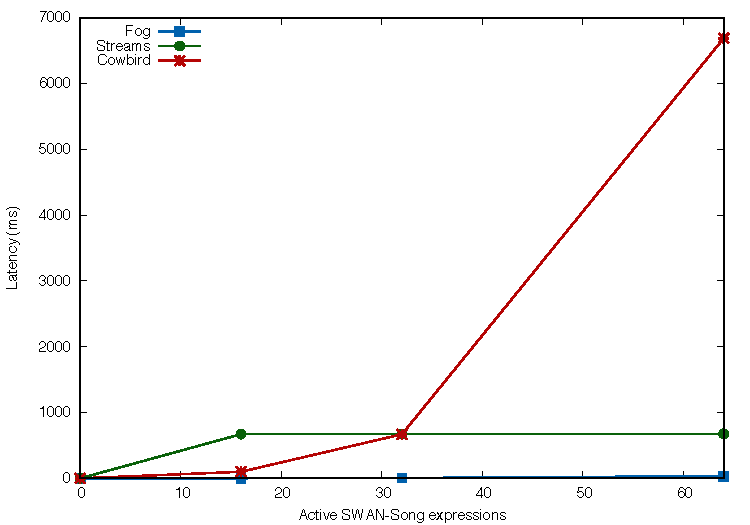
\includegraphics[width=1\textwidth]{images/cowbird_comparison.pdf}
 \caption{SWAN-Song expressions evaluation with sensors that produce fresh data every second. The expressions have the MEAN history reduction mode set and a time window of 5 seconds.}
\label{fig:cowbird_comparison}
\end{figure}
In this test, we compare the original Cowbird framework against the new hybrid architecture. Figure \ref{fig:cowbird_comparison} shows the latency when up to 64 SWAN-Song expressions are evaluated in the original Cowbird cloud framework and in the new Fog and Streams layer. The SWAN-Song expressions evaluated are based on a sound sensor that emits a new data record every second; the history window is 5 seconds. The original Cowbird framework is running on a machine with the same characteristics of a Cowbird Node of the Fog layer. We can notice that the original Cowbird framework with just 64 active SWAN-Song expressions has a latency that is not tolerable for a streaming application.


 \begin{figure}[h!]
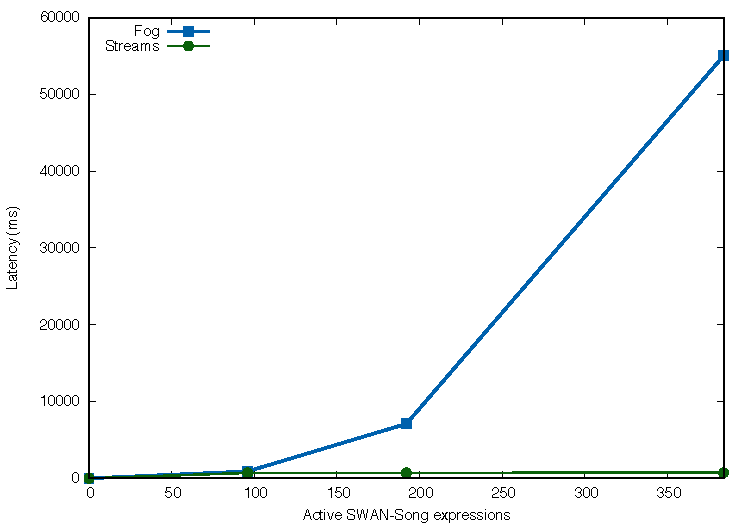
\includegraphics[width=1\textwidth]{images/0_5.pdf}
 \caption{SWAN-Song expressions evaluation with sensors that produce a fresh data record every 500 ms. The expressions have the MEAN history reduction mode set and a time window of 5 seconds.}
\label{fig:0_5}
\end{figure}

 \begin{figure}[h!]
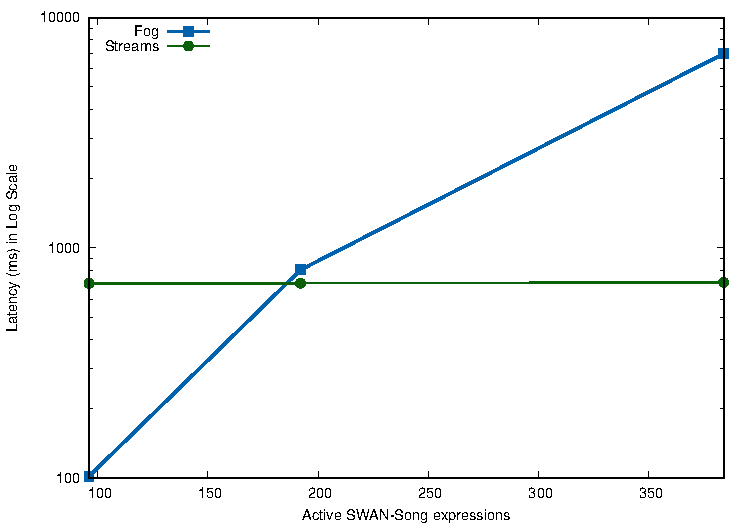
\includegraphics[width=1\textwidth]{images/1_0.pdf}
 \caption{SWAN-Song expressions evaluation with sensors that produce a fresh data record every second. The expressions have the MEAN history reduction mode set and a time window of 5 seconds.}
\label{fig:1_0}
\end{figure}

 \begin{figure}[h!]
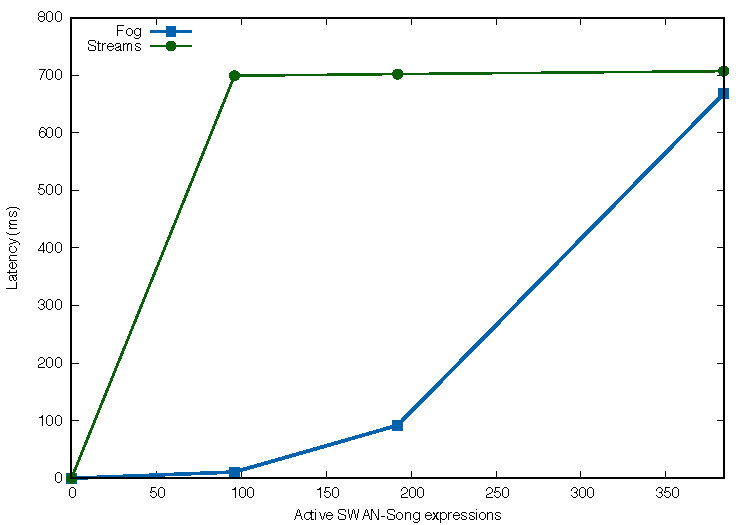
\includegraphics[width=1\textwidth]{images/2_0.pdf}
 \caption{SWAN-Song expressions evaluation with sensors that produce a fresh data record every 2 seconds. The expressions have the MEAN history reduction mode set and a time window of 5 seconds.}
\label{fig:2_0}
\end{figure}

\newpage

 \begin{figure}[h!]
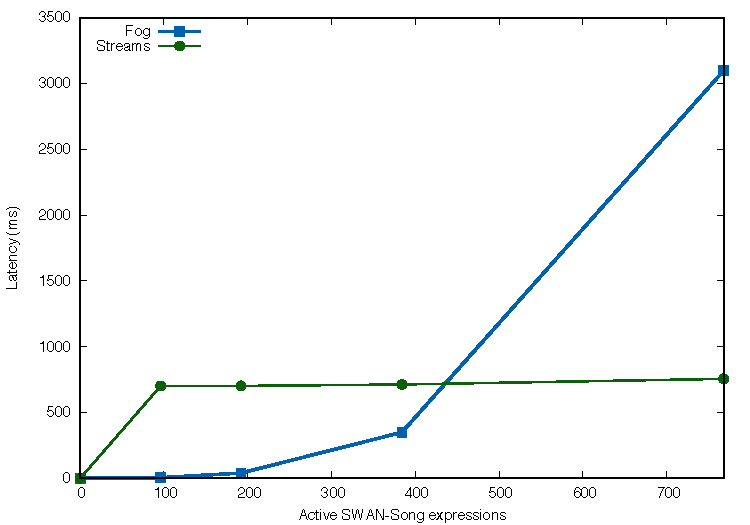
\includegraphics[width=1\textwidth]{images/5_0.pdf}
 \caption{SWAN-Song expressions evaluation with sensors that produce a fresh data record every 5 seconds. The expressions have the MEAN history reduction mode set and a time window of 10 seconds.}
\label{fig:5_0}
\end{figure}


The SWAN-Song expressions evaluated over the Fog layer, instead, have a very low latency (less than 35 milliseconds). This performance is achieved because the sensing and the expression evaluations are distributed over different computing nodes. 

The expressions evaluated in the Streams layer have a certain overhead due the data transmission and communication required between the Fog and the Streams layer through the Kafka broker. %In this particular, in this deployment scenario we have a latency of 700 milliseconds. 

\subsection{Sensing Frequency Tests}
In these tests, we offload a certain number of SWAN-Song expressions characterized by different sensing frequencies.
\paragraph{}
Figure \ref{fig:0_5} shows how the Hybrid-Cowbirds reacts when different loads of SWAN-Song expressions are offloaded to the system. The evaluated expressions use a sensor that produces a new data record every 500 ms and have a history window size of 5 seconds. The evaluation has been done in both the Fog and the Streams layer using the core evaluation implementation. 

Increasing the number of active SWAN-Song expressions in the system drastically boosts the latency when the evaluation is performed entirely in the Fog layer. In fact, many active sensors that produce fresh data records with a high-frequency slow down the SWAN-Song expression evaluations. Active threads that simultaneously need (finite) computing resources for fetching new data records or for computing SWAN-Song expressions have to wait for their turn to access the CPU. Furthermore, each sensor thread has to report the sensed data to an expression evaluation thread. Such communication requires synchronization between the sensing and evaluation threads that introduces a certain overhead.
% In particular, sensor threads require mutual exclusion access 
Hence, extra latency is involved with the increase of many concurrent active sensor threads. 

Offloading the same load of SWAN-Song expressions to the Streams layer leads to way better performance. In fact, even though the number of sensing threads per Cowbird Node increases, each produced value is asynchronously sent through the network to the Streams layer. The Streams layer is capable of evaluating 384 active SWAN-Song expressions with a latency of $\sim$700 milliseconds. 

% However, we noticed a decrease in the system performance when the whole system is executed over a long period of time. The reason for this could be the limited resources assigned to the Kafka cluster. In fact, the Kafka cluster acts as a bottleneck in the architecture. We believe that scaling out the Kafka cluster will let the system to achieve better performance. 

\paragraph{}
Figure \ref{fig:1_0} shows how the system performed with SWAN-Song expressions that use sound sensors that produce data with a lower frequency than the previous test case (i.e. new data record every 1 second). For a better understanding of the plotted data, Figure \ref{fig:1_0} reports the achieved results in logarithmic scale.

In this experimental scenario, the Fog performs relatively better than the Streams layer up to a certain threshold of workload. A lower sensor frequency allows the Fog to be more flexible and efficient in comparison to the previous scenario. Figure \ref{fig:2_0} and \ref{fig:5_0} show that even lower frequency (a new date record  every 2 and 5 seconds respectively) sensors reduce latency required to produce an evaluation result in the Fog layer. 
\paragraph{}
We can conclude that with very high-frequency sensors the SWAN-Song evaluation could be offloaded to the Streams layer even though it involves extra communication overheads. By offloading the evaluation to the Streams layer, the Fog layer can be used exclusively to sense sensor data. However, from Figure \ref{fig:1_0} and Figure  \ref{fig:5_0} we can notice that it also makes sense to offload the expressions evaluation to the Streams layer when the number of active sensor threads drastically increases. 

%Figure \ref{fig:5_0} shows that with a high number of active threads the latency increases in the Streams layer even if the offloaded expressions have a low frequency. As already mentioned, one possible explanation can be that the Kafka cluster runs on a single instance node and this could slow down the flow of the whole system.
% We can also notice that in this test the Streams layer performs better than previous scenarios with sensors that generate data with higher frequency. In this case, the Fog layer publish sensors data to the Streams layer with less frequency reducing the Kafka overhead.

\subsection{Scalability Test}
Figure \ref{fig:5_0_3_nodes} shows the results obtained on deploying the SWAN-Song expressions that use sound sensors that produce a new data record every 5 seconds. The evaluation is performed over a time window of 10 seconds. In this test, we deployed the Fog layer with only 5 nodes. We can see that the Fog layer performs worse than what is shown in Figure \ref{fig:5_0} with the same workload. Cowbird Nodes can be added at run time to \emph{scale out} the Fog layer and accommodate bigger loads of data sensing and evaluation.

 \begin{figure}[h!]
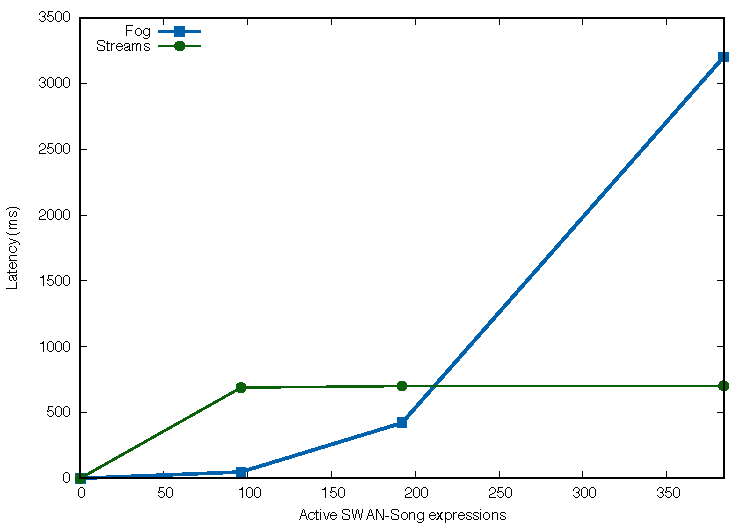
\includegraphics[width=1\textwidth]{images/5_0_3_node.pdf}
 \caption{SWAN-Song expressions evaluation with sensors that produce a fresh data record every 5 seconds over a time window of 10 seconds. The Fog layer uses 5 computing nodes (3 Cowbirds Nodes).}
\label{fig:5_0_3_nodes}
\end{figure}


 \begin{figure}[h!]
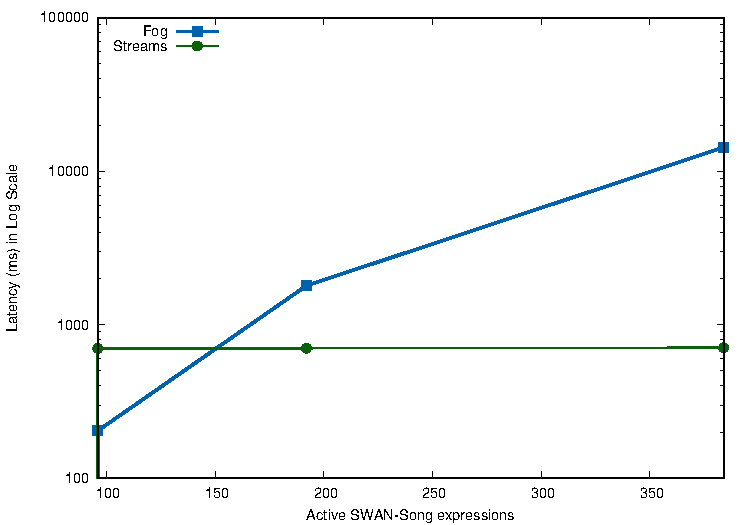
\includegraphics[width=1\textwidth]{images/2_expressions.pdf}
 \caption{SWAN-Song expressions evaluation with two sensors that produce a fresh data record every second over a time window of 5 seconds.}
\label{fig:2_sensors}
\end{figure}

\subsection{Two Sensors Expressions}
We also tested our Hybrid-Cowbirds framework with more complex SWAN-Song expressions. Figure \ref{fig:2_sensors} reports the latency obtained when the system evaluates SWAN-Song expressions composed by two different sensors. For clarity, Figure \ref{fig:2_sensors} reports the achieved latency using logarithmic scale on the y-axis. 

In this experiment, we combined in a SWAN-Song expression the sound sensor with a light sensor that provides information regarding the intensity of the light for a certain area. We designed the expression in order to detect quiet and bright areas. Such an expression is very similar to the SWAN-Song below:
\begin{equation}\label{eq:sound_light_sensor_tristate}
self@sound:value\big\{MEAN, 5000\big\} < 55.0  \text{ \&\& } self@light:value\big\{MEAN, 5000\big\}  > 220.0
\end{equation}

We offloaded the SWAN-Song expression (\ref{eq:sound_light_sensor_tristate}) on our hybrid architecture setting the sensor frequency to a data record per second and the history window to 5 seconds. From Figure \ref{fig:2_sensors} we can notice that the latency obtained by the Fog layer is much higher than what is shown in Figure \ref{fig:1_0}. In both the test cases the sensors data are generated with the same frequency but in this second experiment each expression evaluation has to allocate two different sensing threads.

From Figure \ref{fig:2_sensors} we can also notice that the evaluation in the Streams layer, instead, remains pretty similar to the latency depicted in \ref{fig:1_0}. With up to 384 SWAN-Song expressions the latency of the Streams layer does not encounter any break down.

%\begin{dmath} \label{eq:her}
%self@sound:value\big\{MEAN, 5000\big\} < 55.0 
% 	\text{ \&\& }
% self@light:value\big\{MEAN, 5000\big\}  > 220.0
%\end{dmath}

\subsection{Streaming-Oriented vs Core Implementation}
We performed tests with both the SWAN-Song evaluation strategies implemented for the Streams layer: the \emph{streaming-oriented} and the \emph{core} implementation. As outlined in Chapter 5, the streaming implementation does not keep all the data records generated by sensors but instead it stores only the partial result for each SWAN-Song expression. 

\subsubsection{Streaming-Oriented Storage Efficiency}
We tested the two implementations evaluating sound sensors data with the SWAN MEDIAN history reduction mode over a history window of one hour. Figure \ref{fig:memory_consumption} shows the size of the RocksDB checkpoint directory used by Apache Flink in the Streams layer. Flink periodically records the \emph{state} of the streaming it handles for fault tolerance purposes. After one hour of execution we can notice that the size of the directory used by the \emph{streaming-oriented} evaluation implementation is $\sim$20 times smaller. This can be a good indication of the storage efficiency achieved by the streaming-oriented evaluation implementation.

 \begin{figure}[h!]
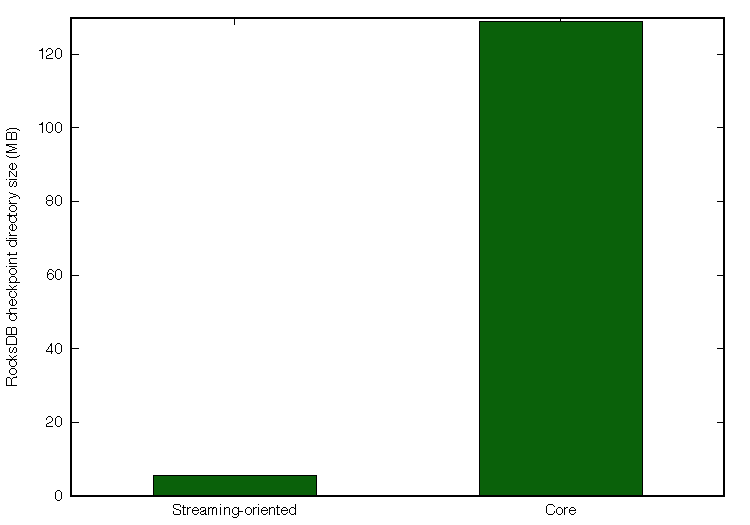
\includegraphics[width=1\textwidth]{images/memory_consumption.pdf}
 \caption{RocksDB checkpoint directory size after one hour evaluation of 768 SWAN-Song expressions that use a sound sensor that produces a data  record every second.}
\label{fig:memory_consumption}
\end{figure}

\subsubsection{Evaluating a Large Number of SWAN-Song Expressions in Cowbird Streams}
We also measured the latency with a very high number of active SWAN-Song expressions evaluated in the Streams layer. Figure \ref{fig:1_0_median} shows a comparison of the latency measured with up to 5,000 SWAN-Song expressions deployed on the Cowbird Streams layer. In this scenario, over a test period of 1 hour each Cowbird Node transmitted over the network $\sim$1.5 GB. The evaluations are performed using both the \emph{streaming-oriented} and the \emph{core} implementation. The expressions use sensor threads that generate new data values every 1 second and have a history window of 5 seconds. We can notice that the two implementations react similarly in terms of latency. However, with a high load of expressions the streaming-oriented implementation seems to perform slightly better than the core evaluation strategy. One possible explanation could be a better streaming state management of the streaming-oriented evaluation strategy. As we have seen the streaming-oriented evaluation optimizes space consumption. Hence, when a result is computed only the partial result has to be decompressed from the RocksDB state backend. Instead, using the  core implementation all the data values involved in the evaluation have to be compressed/decompressed from the state backend. Furthermore, the core evaluation generates more communication traffic within the system. In the core evaluation strategy, expression results are computed continuously as fresh data enter the system. Instead, the streaming-oriented implementation uses \emph{fixed} or \emph{aligned} window mechanisms. 

In this test scenario, we achieved a \emph{throughput} of 5,000 events/s with a latency of $\sim$1.1 seconds. When offloading more than 5,000 expressions we noticed delays in the SWAN-Song expressions evaluation. In particular, we experienced a high CPU usage and a slow down of the outbound network traffic. This leads to an increment of the size of the outgoing message buffers and then to a bigger heap consumption. We also observed a decrease of the Kafka broker performance because of the active traffic between the Fog and the Streams layer. This is a clear symptom that the Fog layer should be scaled-out along with the Kafka instance. 
 \begin{figure}[h!]
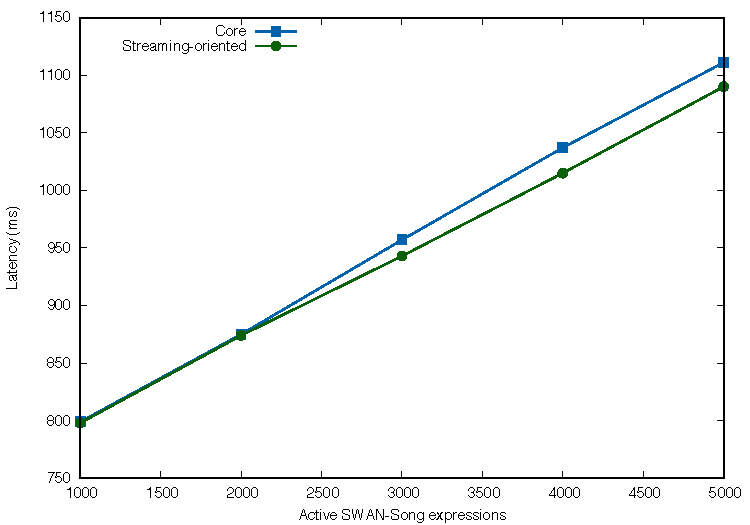
\includegraphics[width=1\textwidth]{images/1f_MEDIAN.pdf}
 \caption{SWAN-Song expressions evaluation with sensors that produce a fresh data record every second. The expressions have the MEDIAN history reduction mode set and a time window of 5 seconds.}
\label{fig:1_0_median}
\end{figure}


\section{Discussion}
In this section we described some of the tests we performed on our Hybrid-Cowbirds architecture. From the results of our experiments emerge that in some scenarios it makes sense to combine the data sensing and  the SWAN-Song evaluation in the Fog layer. As we have seen in the \emph{Scalability Test} described in Subsection 6.4.3, the Fog layer can scale out easily in order to accommodate an increasing number of SWAN-Song expression evaluation requests. However, experimental results outlined in Subsection 6.4.2 highlight that after a certain threshold, the Fog layer cannot handle anymore the burden of evaluating the sensed data in scenarios characterized by \emph{high-frequency} sensors.
% However, according to the results obtained from our \emph{Sensing Frequency Tests} is that in situations characterized by \emph{high-frequency} sensors the Fog layer cannot handle anymore the burden of evaluating the sensed data. In these contexts, the evaluation can be simply offloaded to the Streams layer. 
The Streams layer along with the sensing capabilities provided by the Fog layer can guarantee real-time performance for data evaluations.

Furthermore, not only SWAN-Song expressions characterized by high-frequency sensors can be offloaded to the Streams layer. Some applications require sensor data collected over long time windows such as hours or even days. Such scenarios could certainly benefit from the Streams layer. In the original design of the SWAN framework, all the sensor values are kept in memory. Hence, the memory heap could be easily saturated if many long-running SWAN-Song expressions are allocated. %As a matter of fact, with 64 active sound sensor threads that produce a float data value every second the Java default heap size is saturated in less than 2hrs u .

Long-running SWAN-Expressions could be offloaded to the Streams layer that runs on a cluster that is usually characterized by Terabyte of memory and Petabyte of disk.  

\paragraph{}
The Kafka broker is the backbone of the Hybrid-Cowbirds architecture. In actual deployment, it should be characterized by multiple nodes and it should scale-out along with the Fog layer in order to prevent it from becoming a communication bottleneck between the Fog and the Streams layer as happened in our \emph{Evaluating a Large Number of SWAN-Song Expressions in Cowbird Streams} test (Subsection 6.4.5). 

\paragraph{}
We tested the \emph{streaming-oriented} evaluation realized for the Streams layer in our \emph{Streaming-Oriented vs Core Implementation} tests (Subsection 6.4.5). We demonstrated that it is more efficient than the core implementation when storing the data streaming state. This could bring benefits when evaluating long-running expressions characterized by a relatively big internal streaming state.

\paragraph{}
In a Fog computing context, the tested setup is not very realistic. In fact, all the architecture components run in the same SURFsara data center. As already mentioned in Chapter 5, the architecture could be geographically distributed putting the Fog layer closer to the user. In such scenario, sensor evaluation capabilities will be close to the data generation and to the users. This approach makes possible the definition of a general purpose platform for evaluating smartphone and IoT sensors that would be ready to meet the Fog computing concept. Such a platform would be indeed characterized by low latency and high availability.